\section{Theory}
\markright{Theory}

Diode clipper circuits are used to limit the amplitude of an input waveform by allowing current to pass only in one direction. In a positive clipper, the diode conducts during the positive half-cycle and cuts off the output at a small forward threshold, while in a negative clipper the opposite half-cycle is removed. The operation of these circuits is illustrated in the figures stored in the theory folder \textit{lab-05/assets/theory}, and the corresponding wave-shaping behavior is discussed in \cite{lab_05_boylstad}.

\begin{figure}[H]
  \centering
  \begin{subfigure}[b]{0.45\textwidth}
    \centering
    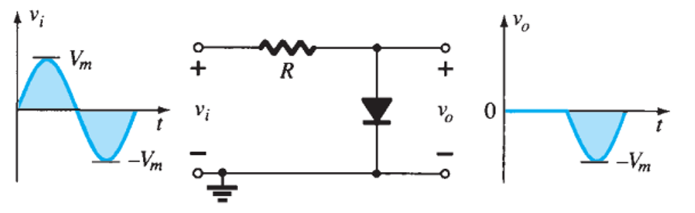
\includegraphics[width=\linewidth]{lab-05/assets/theory/positive-clipper.png}
    \caption{Positive clipper circuit and waveform.}
  \end{subfigure}
  \hfill
  \begin{subfigure}[b]{0.45\textwidth}
    \centering
    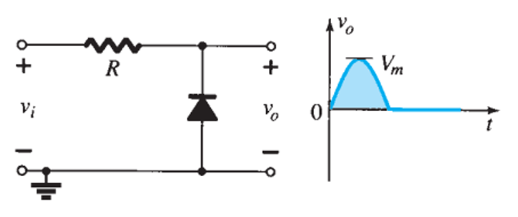
\includegraphics[width=\linewidth]{lab-05/assets/theory/negative-clipper.png}
    \caption{Negative clipper circuit and waveform.}
  \end{subfigure}
  \caption{Unbiased diode clipper circuits and their output behavior.}
  \label{lab05_fig:unbiased_clippers}
\end{figure}

When a DC bias source is connected in series with the diode, the clipping level shifts from zero to the bias voltage. This enables the circuit to clip at a desired positive or negative level, which is useful for waveform shaping and signal protection. The biased configurations shown in the same theory folder demonstrate how the output waveform is altered when the diode is forward-biased or reverse-biased with an external source, as explained in \cite{lab_05_boylstad}.

\begin{figure}[H]
  \centering
  \begin{subfigure}[b]{0.45\textwidth}
    \centering
    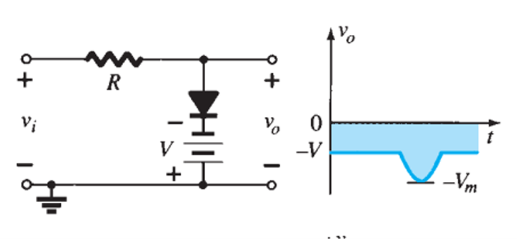
\includegraphics[width=\linewidth]{lab-05/assets/theory/negative-bias-positive-clipper.png}
    \caption{Positive clipper with negative bias.}
  \end{subfigure}
  \hfill
  \begin{subfigure}[b]{0.45\textwidth}
    \centering
    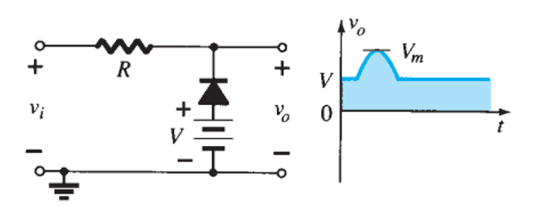
\includegraphics[width=\linewidth]{lab-05/assets/theory/positive-bias-negative-clipper.png}
    \caption{Negative clipper with positive bias.}
  \end{subfigure}
  \caption{Biased diode clipper circuits with shifted clipping levels.}
  \label{lab05_fig:biased_clippers}
\end{figure}
